%=======================
%Бабаев

\section{Расчет относительных дисперсий намагниченности и восприимчивости в неупорядоченной модели Изинга}




%\subsection{Аннотация}
%
%
%На основе метода Монте-Карло рассчитаны относительные дисперсии намагниченности  $R_m$ и восприимчивости $R_\chi$  в трехмерной неупорядоченной спиновой решеточной модели Изинга в зависимости от концентрации спинов. Показано, что внесение беспорядка в виде немагнитных примесей в трехмерную модель Изинга приводит к отличным от нуля значениям для $R_m$ и $R_\chi$.




\subsection{Трехмерная неупорядоченная модель Изинга с примесями}

При численных исследованиях, разбавленных изингоподобных систем следует иметь в виду, что есть серьезные основания предполагать наличие зависимости критических параметров от способа реализации беспорядка в исследуемой модели.

Например, в работах \cite{ph2_1,ph2_2} было обнаружено, что беспорядок, реализованный каноническим способом (фиксацией доли магнитных узлов), ведет к результатам, отличным от случая, когда беспорядок реализовался способом большого канонического типа (доля магнитных узлов в каждой примесной конфигурации флуктуирует), хотя исследования \cite{ph2_3} проведенные ренормгрупповыми методами такое поведение объяснило различием конечно-размерных эффектов в этих двух типах разбавления.

По-видимому, строгое исследование таких закономерностей в ближайшее время возможно лишь на основе данных численного эксперимента и практически невозможно другими методами. Отметим также, что анализ результатов работы \cite{ph2_4} полученных на трехмерной разбавленной модели Изинга, в которой вмороженный беспорядок внесен в виде случайных ферромагнитных связей, привел авторов к выводу, что в большей части критической области доминирует кроссовер от показателей чистой модели к показателям неупорядоченной модели.

В последнее время предметом изучения методом Монте-Карло стали и другие реализации беспорядка. В качестве обобщения трехмерной разбавленной модели Изинга в работах \cite{ph2_5,ph2_6} исследовалась термически разбавленная модель Изинга. В этом случае реализация распределения вакансий определялась из локального распределения спинов чистой модели Изинга в критической точке.

Оказалось, что критические свойства этой модели сильно отличаются от трехмерной разбавленной модели Изинга в которой беспорядок содержится в виде вмороженных немагнитных примесей или в виде случайных ферромагнитных связей и соответствуют теоретическим предсказаниям для скоррелированного на больших расстояниях беспорядка \cite{ph2_7}.

Отметим, что поведение термодинамических критических параметров неупорядоченных моделей при различных реализациях беспорядка в виде немагнитных примесей в широком интервале изменении концентрации примесей $c_{imp}$, $c_{imp}=1-p$, c соблюдением единой методики до настоящего времени исследовано недостаточно полно. Не выяснены особенности распределения термодинамических параметров по соответствующему ансамблю.

В связи с этим нами исследуется проблема самоусреднения термодинамических критических параметров в трехмерной неупорядоченной модели Изинга на основе метода Монте-Карло.






\subsection{Результат исследования}


Рассчитаны относительные дисперсии намагниченности  $R_m$ и восприимчивости $R_\chi$  для трехмерной неупорядоченной спиновой решеточной модели Изинга в зависимости от концентрации спинов.  На рисунках \ref{phys2-pic-1} и \ref{phys2-pic-2} представлены зависимости
\begin{equation*}
  R_m = \frac{\overline{m^2(L)}-\overline{m(L)}^2}{\overline{m(L)}^2}
\end{equation*}
\begin{equation*}
  R_\chi = \frac{\overline{\chi^2(L)}-\overline{\chi(L)}^2}{\overline{\chi(L)}^2}
\end{equation*}
от размеров $L$ систем. Эти данные позволяют судить об ошибках, связанных с размерами изучаемых систем.




\begin{figure}[H]
	\centering
	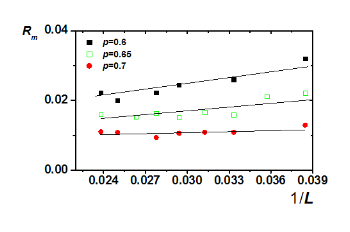
\includegraphics[width=0.5\linewidth]{content/sections/images/phys2-1}
	\caption{Зависимость относительных дисперсий намагниченности $R_m$ от обратных размеров спиновой системы при $T(p)=T_c(p)$.}
	\label{phys2-pic-1}
\end{figure}

\begin{figure}[H]
	\centering
	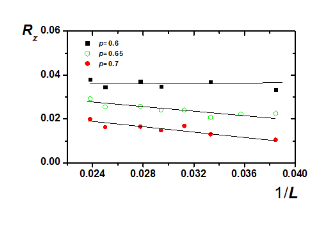
\includegraphics[width=0.5\linewidth]{content/sections/images/phys2-2}
	\caption{Зависимость относительных дисперсий намагниченности $R_{\chi}$ от обратных размеров спиновой системы $1/L$ при $T(p)=T_c(p)$.}
	\label{phys2-pic-2}
\end{figure}


Отметим, что наши значения $R_m$, $R_\chi$ заметно отличаются от аналогичных данных, полученных в работе \cite{ph2_4} при большом каноническом способе реализации беспорядка (магнитная доля узлов флуктуирует в зависимости от концентрации $p$), а также и с предположением теории ренормализационной группы  $R_m / R_\chi = 1/4$. В указанной работе рассматривался только канонический способ реализации беспорядка и при концентрации спинов $p=0.7$ отношения $R_m / R_\chi =0.502, 0.555, 0.559$ для $L=44, 40, 36$ соответственно.

Эти отношения находятся в достаточно хорошем согласии с отношением \linebreak $R_m / R_\chi \equiv 2/5$, полученное в работе \cite{ph2_1} для беспорядка реализованного каноническим способом при концентрации спинов $p=0.6$. Отметим, что различие наших данных с данными работы \cite{ph2_4}, по-видимому, обусловлено различными конечно-размерными эффектами в этих двух различных типах разбавления.


Нами также проводилась обработка этих данных с учетом поправок к КРС. Учет которых особенно важен из-за очень медленного приближения $R_\chi$ к своему универсальному асимптотическому значению \cite{ph2_3}. Для этого нами использовалось следующее выражение
\begin{equation}
  R_\chi(L) = R_X(\infty)+A^C L^{-(\phi/\nu)_{random}}
\end{equation}
где $(\phi/\nu)_{random}$ --- показатель поправки к скейлингу, $A^C$ --- некоторая постоянная зависящая от степени разбавления.
Была также получена экстраполяция МК данных для среднеквадратичных отклонений намагниченности $R_m$ на $L \rightarrow \infty$  для всех рассмотренных концентраций спинов $p$.

В качестве поправки к ведущему члену скейлинга $\omega = (\phi/\nu)_{random}$  следуя работам \cite{ph2_8,ph2_9} мы брали значения в разбавленной области $(p\le0.95)$ $\omega=0.36(6)$.
Как видно из приведенных рисунков учет поправки позволяет выйти на асимптотический режим и корректно оценить универсальные параметры ($p$-indepent universal value).

Следует отметить, что в сильно разбавленной области $(p\le0.7)$ наблюдается заметное отклонение МК данных соответствующих малым размерам системы от прямой. Эти значения при экстраполяции на $L \rightarrow \infty$    нами не учитывались.






%\subsection{Заключение}
%
%
%На основе кластерного алгоритма Вольфа метода Монте-Карло рассчитаны относительные дисперсии для намагниченности $R_m$, и восприимчивости $R_\chi$ в широком интервале разбавлений $c$, $c=1-p$.
%Показано, что внесение вмороженного беспорядка в чистую трехмерную модель Изинга приводит к отличным от нуля значениям для $R_m$, и для $R_\chi$, что указывает на плохое самоусреднение термодинамических параметров в разбавленных системах.


